\documentclass[tikz,border=10pt]{standalone}
\usetikzlibrary{positioning,arrows.meta}
\definecolor{eventFill}{HTML}{FFE0B2}
\definecolor{eventBorder}{HTML}{FB8C00}
\definecolor{subjectFill}{HTML}{C8E6C9}
\definecolor{subjectBorder}{HTML}{4CAF50}
\definecolor{observerFill}{HTML}{E1BEE7}
\definecolor{observerBorder}{HTML}{9C27B0}

\begin{document}
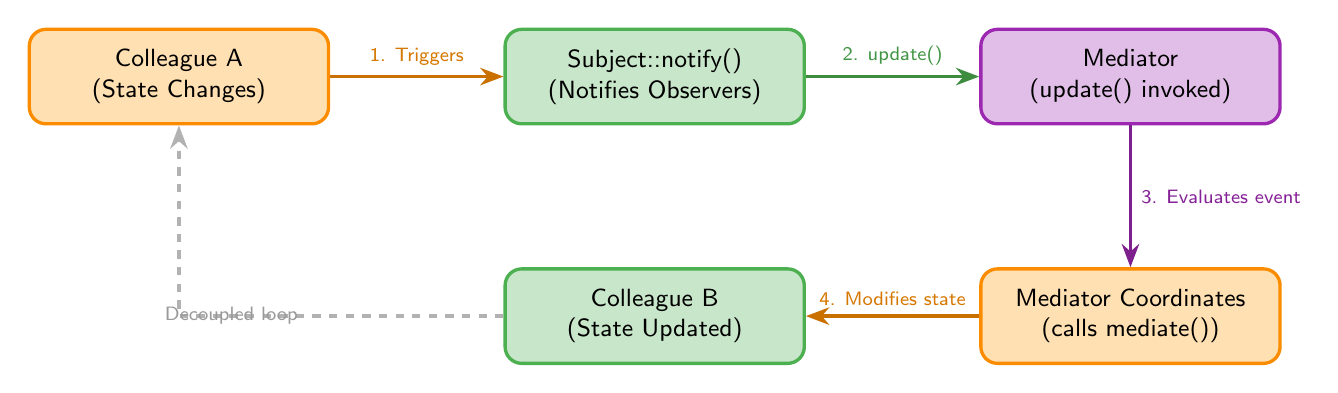
\begin{tikzpicture}[
    block/.style={
        rectangle, draw,
        minimum width=3.8cm, minimum height=1.2cm,
        align=center,
        text centered, rounded corners=6pt,
        line width=1.2pt, font=\sffamily\small
    },
    arrow/.style={-{Stealth[scale=1.0]}, line width=1.2pt}
]
  % Nodes
  \node[block, fill=eventFill, draw=eventBorder] (change) {Colleague A\\(State Changes)};
  
  \node[block, fill=subjectFill, draw=subjectBorder, right=2.2cm of change] (notify) {Subject::notify()\\(Notifies Observers)};
  
  \node[block, fill=observerFill, draw=observerBorder, right=2.2cm of notify] (mediator) {Mediator\\(update() invoked)};
  
  \node[block, fill=eventFill, draw=eventBorder, below=1.8cm of mediator] (coordinate) {Mediator Coordinates\\(calls mediate())};
  
  \node[block, fill=subjectFill, draw=subjectBorder, left=2.2cm of coordinate] (target) {Colleague B\\(State Updated)};

  % Flow arrows
  \draw[arrow, draw=eventBorder!80!black] (change) -- (notify)
      node[midway, above, font=\sffamily\scriptsize, text=eventBorder!85!black] {1. Triggers};
      
  \draw[arrow, draw=subjectBorder!80!black] (notify) -- (mediator)
      node[midway, above, font=\sffamily\scriptsize, text=subjectBorder!85!black] {2. update()};
      
  \draw[arrow, draw=observerBorder!80!black] (mediator) -- (coordinate)
      node[midway, right, font=\sffamily\scriptsize, text=observerBorder!85!black] {3. Evaluates event};
      
  \draw[arrow, draw=eventBorder!80!black] (coordinate) -- (target)
      node[midway, above, font=\sffamily\scriptsize, text=eventBorder!85!black] {4. Modifies state};

  % Loop back dotted line to indicate decoupled communication loop
  \draw[arrow, draw=gray!60, dashed] (target) -| (change)
      node[pos=0.3, left, font=\sffamily\scriptsize, text=gray!80] {Decoupled loop};

\end{tikzpicture}
\end{document}
